% Chapter 1

\chapter{The curve graph of a surface} % Main chapter title

\label{Chapter1} % For referencing the chapter elsewhere, use \ref{Chapter1} 

\lhead{Chapter 1. \emph{The curve graph of a surface}} % This is for the header on each page - perhaps a shortened title

%----------------------------------------------------------------------------------------

The study of surfaces in a strictly topological viewpoint has made us to forgot significant information about them. A way to revert this is to attach a group to it, the \textbf{mapping class group} of the surface. It is denoted by $Mod(S)$ and encode the \textit{symmetries} of the surface. This group is defined as the set of isotopy classes of orientation-preserving homeomorphisms of $S$. In the first section of this chapter we give the formal definition of this group and establish the very important role of this concept in Mathematics. 

A widely accepted idea is that, Mathematics can be thought as a story of groups and actions. Taken this point of view, the \textbf{curve complex} of the surface, denoted by $C(S)$ appears naturally in the study of $Mod(S)$. It is a simplicial complex that encodes intersection patterns of simple closed curves in $S$. We focus part of the discussion in the relationship between the algebraic structure of $Mod(S)$ and the combinatorial topology of $S$.

Many of the progress in understanding $Mod(S)$ has been possible by a well-known comparison among two very important classes of groups: arithmetic groups and mapping class groups. In this parallelism panorama arises the desire for an equivalent, until some extent, of the Margulis Superrigidity for mapping class groups.

In the last section of this chapter we settled the bases that allow us to understand a notion of rigidity in graph theory. An approach called \textit{rigid expansions}, see \cite[Aramayona 16]{rigidExpJA} and \cite[Hernandez 16]{rigidExpJH}, allows us to build up subgraphs preserving the rigidity property and it is compatible with the stochastic scheme outlined in chapter 2.
 
Many results and definitions in this chapter where extracted from \cite[Farb]{Farb}. They are quite popular and equivalents can easily be find in the literature, however they are written here to establish nomenclature. Familiarity with basic concepts will be assumed.

\section{Mapping class group of a surface}

We have the following fundamental, well-known result about surfaces.

\begin{theorem}[Classification of surfaces]\label{CST}
Any closed, connected, orientable surface is homeomorphic to the connect sum of a 2-dimensional sphere with $g \geq 0$ tori. Any compact, connected, orientable surface is obtained from a closed surface by removing $b \geq 0 $ open disks with disjoint closures. Even more, the set of homeomorphism types of compact surfaces is in bijective correspondence with the set $\{ (g, b) : g, b \geq 0\}$.
\end{theorem}

We are so familiarize with this result that we usually forget what is saying. It seems like, in the eyes of a topologyst, there is nothing much interesting about surfaces, but this is because we are forgetting all the geometric information about them. $Mod(S)$ helps to recover this data, the magic happens when this group acts on the \textbf{Teichmüller space} of $S$, that is the space of hyperbolic metrics on $S$ up to isotopy. A central result is that this action is properly discontinuous and the quotient space $M(S) = Teich(S)/ Mod(S)$ is the \textbf{moduli space of Riemannian surfaces homeomorphic to $S$}. The space $M(S)$ is a essential object in mathematics and the group $Mod(S)$ encodes most of the topological features of $M(S)$.

$Mod(S)$, $Teich(S)$, and $M(S)$ can be found in a lot of different contexts in mathematics: hyperbolic geometry, algebraic geometry, combinatorial group theory, symplectic geometry, 3-manifold theory, dynamics and so on. The algebraic structure of $Mod(S)$, the geometry of $Teich(S)$, and the topology of $M(S)$ are just the strands which are used to weave the rich tapestry of the topology of the surface.

Before we continue, let's establish some nomenclature. The $g$ in \ref{CST} is called the \textit{genus} of the surface and the $b$ is the number of \textit{boundary components}. One way to obtain a non-compact surface from a compact one is to remove $m$ points from the interior of it; in this case, we say that the resulting surface has $m$ punctures. For now on, unless otherwise specified, we will be thinking in compact, connected, oriented surfaces that are possibly punctured (in this case they ceases to be compact). Therefore, we can specify the surfaces by the triplet $(g, b, m)$. We will denote by $S_{g,m}$ a surface of genus $g$ with $m$ punctures and empty boundary; such a surface is homeomorphic to the interior of a compact surface with $m$ boundary components. Also, for a closed surface of genus $g$, we will abbreviate $S_{g,0}$ as $S_{g}$ and $\partial S$ denote the (possibly disconnected) boundary of $S$.

There are a number of definitions for the mapping class group of a surface. We will be working with the following:

\begin{defini}
Let $S$ be a surface, the \textbf{mapping class group} of $S$, denoted by $Mod(S)$ is the following quotient:
$$Mod(S)=Homeo^{+}(S)/Homeo_{0}(S)$$
where $Homeo^{+}(S)$ is the group of orientation-preserving, homeomorphisms of $S$, that are the identity on the boundary, this group can be endowed with the compact-open topology. $Homeo_{0}(S)$ is the subgroup formed by homeomorphisms of $S$ which are isotopic to the identity, i.e. the connected component of the identity with this topology.
\end{defini}

We could consider diffeomorphisms instead of homeomorphisms, or homotopy classes instead of isotopy classes, this will result in isomorphic groups, see \cite[Farb 41]{Farb} for details in why we can do this. Summarizing, we can find the following variations in the definition of $Mod(S)$:

\centerline{\begin{tabular}{ rcl }
$Mod(S)$ & $=$ & $\pi_{0}(Homeo^{+}(S, \partial S))$\\
 & $\approx$ & $Homeo^{+}(S,\partial S)/\textit{homotopy}$\\
 & $\approx$ & $\pi_{0} (\textit{Diff}^{+}(S,\partial S))$\\
\end{tabular}}

where $\textit{Diff}^{+}(S, \partial S)$ is the group of orientation-preserving diffeomorphisms of $S$ that are the identity on the boundary. It can be taken to be either smooth homotopy relative to the boundary or smooth isotopy relative to the boundary.

A lot of work had been made to describe the types of elements in $Mod(S)$. Thanks to the Thurston's classification theorem there is a characterization of the homeomorphisms of a compact orientable surface. This classification is useful to describe the curve graph which will be analyzed in the next section.

\subsection{Nielsen–Thurston classification}
Given a homeomorphism $f: S \to  S$, there is a map $g$ isotopic to $f$ such that at least one of the following holds:

\begin{itemize}
\item $g$ is periodic, i.e. some power of $g$ is the identity;
\item $g$ preserves some finite union of disjoint simple closed curves on $S$ (in this case, g is called reducible); or
\item $g$ is pseudo-Anosov.
\end{itemize}

The definition of a \textbf{pseudo-Anosov map} relies on the notion of a measured foliation, a geometric structure on $S$. It consists of a singular foliation and a measure in the transverse direction (i.e. that is constant in transverse arches). For the full definition of pseudo-Anosov elements and the proof of this theorem we can refer to \cite[Farb, Chapter 13]{Farb}.

The study of mapping class groups is a wide and challenging area by it self. It is outside of the interests of this thesis to review the details and repercussions of this vastly field. Yet, there are a number of known properties of $Mod(S)$ that it would be nice to have in mind in further work, although different tools might be required.

\begin{itemize}
\item Finitely generated and presented
\item It has a subgroup of finite index which doesn't have torsion.
\item $Mod(S_{g,m}) \cong Out(\pi_{1}(S_{g,m})$
\item $H_{1}(Mod(S_{g,m}), \Z) = 1$ when $(g\geq3, m=0)$
\end{itemize}

\section{Curve graph}

\subsection{Simple closed curves}

\begin{defini}
A \textbf{closed curve} in a surface $S$ is a continuous map $\S^{1}\to S$, is called \textbf{simple} if the map is injective. We will usually identify a closed curve with its image in $S$. A closed curve is called \textbf{essential} if it is not homotopic to a point, a puncture, or a boundary component.
\end{defini}
Among the adjectives that a curve can acquired we have the following:
\begin{itemize}
    \item $\alpha$ is \textbf{separating}, if $S-\alpha$ has two components, otherwise it is called \textbf{non separating}.
    \item It is called \textbf{essential} if no component of $S- \alpha$ is a disk.
    \item It is \textbf{non-peripheral} if no component of $S - \alpha$ is an annulus. 
\end{itemize}

We are interested in \textbf{essential} and \textbf{non-peripherial} curves, they will be assumed in this sense, unless otherwise specified.

The idea behind the construction of the curve graph is to stratify the set of homotopy classes of curves on a surface. For this to make sense we define the \textbf{geometric intersection number} between free homotopy classes $a$ and $b$ of simple closed curves in a surface $S$. This is defined to be the minimal number of intersection points between a representative curve in the class $a$ and a representative curve in the class $b$:
$$i(a,b) = min \{ |\alpha \cap \beta| : \alpha \in a, \beta \in b \}$$
It is convenient to adopt a slight abuse of notation by writing $i(\alpha, \beta)$ for the intersection number between the homotopy classes of simple closed curves $\alpha$ and $\beta$. It is useful to think that this number can be calculate by finding representatives $\alpha$ and $\beta$ that realize the minimal intersection in their homotopy classes, so that $i(a, b) = |\alpha \cap \beta|$. When this is the case, we say that $\alpha$ and $\beta$ are in minimal position. Although the geometric intersection number is a useful and intuitive invariant it is not always easy to compute, whenever this is the case we can appeal to the algebraic intersection number. For a further discussion of this see \cite[Farb]{Farb}

\subsection{The curve graph}

\begin{defini}
The \textbf{curve graph} $\Gamma(S)$ of a surface $S$ is constructed by the following data:
\begin{itemize}
\item \textbf{Vertices}. There's a vertex in $\Gamma(S)$ for every isotopy class of essential closed curves in $S$.
\item \textbf{Edges}. There's an edge between the corresponding vertices of isotopy classes $a$ and $b$ whenever $i(a,b)=0$.
\end{itemize}
\end{defini}

\begin{defini}
The \textbf{curve complex of the surface}, $C(S)$ is defined to be the flag complex of the curve graph just defined.
\end{defini}

\section{Properties of the curve graph}
The goal of this sections is to enumerate known properties of the curve graph, this will be useful to establish the appropriate parameters in the probabilistic model. Notice that the construction of the curve complex is completely determined by the curve graph, hence the probabilistic models can work in the same sense. Lets keep in mind the following exceptional cases they are responsible for the conditions stated in the hypothesis of the following theorems for $g$ and $n$. For $ S^2, S_{0,1}, S _{0,2}, S_{0,3} $ the curve graph is empty and for  $ T^{2} $, $ S_{1,1}$ and $ S_{0,4}$ is a countable disjoint union of points.

\subsection{Cardinality of the number of vertices}
\begin{theorem}
If $g\geq 1$ or $n\geq 4$ then the set of vertices in $\Gamma(S_{g,n})$ is countably infinite.
\end{theorem}

It is well known that for $T^{2}$ there is an explicit identification for the isotopy classes of essential curves with the rational numbers. In this case there aren't disjoint curves, the following figure can help to convince us of this.
\vspace{1cm}
\begin{figure}[h!]
	\centering
	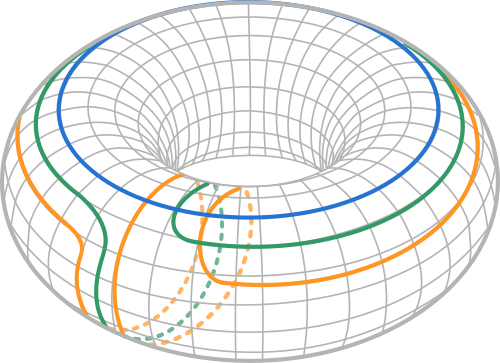
\includegraphics[scale=0.5]{Figures/Torus.png}
	\caption{$T^{2}$ with representatives of typical elements of curves}
\end{figure}

This identification can be seen as the induction basis. The induction step over $g$ comes from splitting the surface, by induction hypotheses none of the resulting surfaces can have a non-countable number of classes of curves.

\subsection{Connectivity}
\begin{theorem}
If $3g+n\geq 5$, then $\Gamma(S_{g,n})$ is connected.
\end{theorem}

To proof this theorem we can show that, for any two isotopy classes $a$ and $b$ of simple closed curves in $s_{g,n}$ exists a sequence of isotopy classes
$$a=c_{1},\dots,c_{k}=b$$
where $i(c_{i},c_{i+1})=0$, this can be done proceeding by induction over $i(a,b)$. The full proof of this theorem can be found in \cite[Farb p.~93]{Farb} 

\subsection{Locally infinity}
\begin{theorem}
If $3g+m\geq 5$, then $\Gamma(S_{g,n})$ is locally infinity.
\end{theorem}
The idea behind the proof is that given any $\alpha \in \Gamma(S)$ we can construct a family of isotopy classes of curves which are disjoint to $\alpha$. The following picture gives us an intuitive idea on how to do this whenever there is enough holes.
\vspace{1cm}
\begin{figure}[h!]
	\centering
	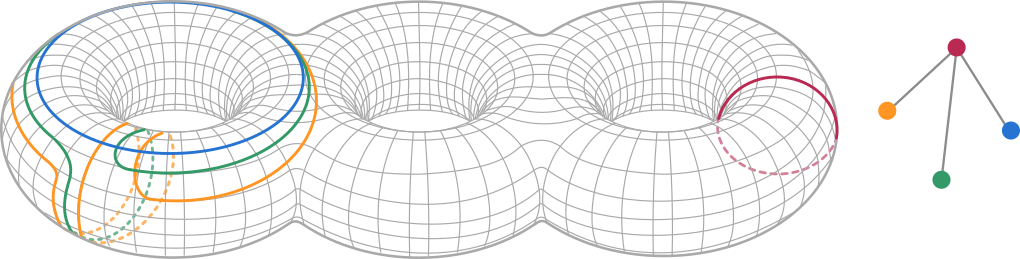
\includegraphics[scale=0.6]{Figures/Locally-infinite.png}
	\caption{$S_{3}$ with typical representative curves which exemplify the locally infinity property}
\end{figure}

For the complete argument, let $\alpha$ be any simple closed curve on $S$, the surface $S-\alpha$ which we obtain by cutting $S$ open along $\alpha$ contains at least one connected component of Euler characteristic at most $-2$, this is guaranteed by the $3g+m\geq 5$ condition. Such component contains infinitely many distinct homotopy classes of simple closed curves disjoint from $\alpha$.

\subsection{Clique number}
A \textbf{clique} in a graph $G$ is a complete subgraph of $G$. The clique number $cl(G)$ of a graph $G$ is the maximum order of a clique of $G$.

\begin{theorem}
If $3g+n\geq 5$, then $3g - 3 + m$ is the clique number of $\Gamma(S_{g,m})$.
\end{theorem}

$3g-3+m$ is the number of curves in a pants decomposition of $S$, i.e. a maximal collection of disjoint, not freely homotopic, essential, simple closed curves which decompose $S$ into $2g-2+m$ open subsurfaces homeomorphic to a thrice punctures sphere. For a full proof of this well-known fact refer to \cite[Hatcher]{Pants}

\vspace{1cm}
\begin{figure}[h!]
	\centering
	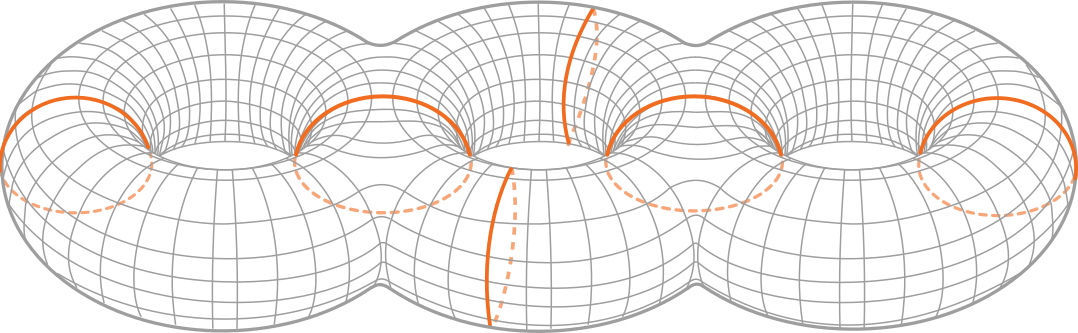
\includegraphics[scale=0.5]{Figures/Pantalones.png}
	\caption{Exemplification of a pants decomposition of a surface}
\end{figure}

\subsection{Infinite Diameter}
\begin{theorem}
If $3g+m\geq 5$ then $diam(\Gamma(S)) = \infty$
\end{theorem}

The proof for this theorem relies on the fact that for any pseudo-Anosov element $h \in Mod(S)$, any $\gamma \in V(\Gamma(S))$ and any $k\in \Z$
$$d_{C}\Big(h^{k}(\gamma), \gamma\Big) \geq c|k|$$
This provide the infinite diameter property. For details, refer to \cite[Masur and Minsky]{Masur}

The curve graph and the curve complex are fundamental tools in the study of the surfaces. There are a number of known properties of them that it would be nice to have in mind to improve probabilistic models in further work.

\begin{enumerate}
\item $C(S)$ is hyperbolic
\item In the infinite case $diam(\Gamma(S))= 2$
\item There's an isomorphism between $Mod(S)$ and $Aut(C(S))$, except when $(g,m) \in \{(1,2), (1,1), (2,0), (0,4)\}$
\end{enumerate}

\section{Rigidity in graphs}

The intention of this section is to track down the motivation to do rigid expansions and give the required definitions.

As mention in the introduction of the chapter, rigidity appears in the mapping class group context in light of its comparison with arithmetic groups. In \cite[Aramayona, S.]{rigidityJA} we can find a survey on the search of an analogue for the Margulis Superrigidity theorem. In this article, they provide three different perspectives: a Lie theoretical, a geometric and a folkloric one.

The Lie theoretic version says that every homomorphism $Mod(X) \to Mod(Y)$ is induced by a homomorphism between the associated groups of diffeomorphisms with compact support disjoint from the boundary $\textit{Diff}_{c}(X) \to \textit{Diff}_{c}(Y)$.

A direct formulation of geometric superrigidity cannot hold when the moduli space is endowed with any reasonable metric. However, there are ways to turn this around, saying that every (irreducible) homomorphism between mapping class groups induces a holomorphic map between the corresponding moduli spaces.

The folkloric version of Mostow and Margulis superrigidity claims that the only homomorphisms between lattices are the \textit{“obvious ones”}, in the $Mod(S)$ context this will mean that if we consider $X$ and $Y$, under suitable conditions, then every homomorphism $Mod(X) \to Mod(Y)$ will be induced by a manipulation of the underlying surfaces. 

A result due to Ivanov \cite{celebratedIvanov}, Korkmaz \cite{celebratedKorkmaz} and Luo \cite{celebratedLuo}, asserts that, excluding few well-understood cases, the curve complexes are simplicially rigid. This means that the group $Aut(C(S))$ of simplicial automorphisms of $C(S)$ is isomorphic to the extended mapping class group. This result is sometimes interpreted as a proof that \textbf{the automorphisms  of  the  curve  complex  are  all geometric}.

In the aim to generalize this result to broader types of simplicial self-maps, in \cite[Aramayona, Leininger - 13]{finiteRigidSetsJA} was introduced the concept of \textbf{rigid sets} in the curve complex. Suppose that $S$ is different from $S_{1,2}$,  $Y \subset C(S)$ it is called \textbf{rigid} if for every locally injective simplicial map $\Phi  : Y \to C(S)$ there exists $h \in Mod{\ast}(S)$ with $h|_{Y} = \Phi$, unique up to the pointwise stabilizer of $Y$ in $Mod^{\ast}(S)$.

Later on in \cite[Aramayona, Leininger - 13]{exhaustionByRigidSets}, they developed a method for enlarging subgraphs and proved that for almost all surfaces of finite topological type, there exists an \textbf{increasing sequence of finite rigid sets} that exhaust the curve graph of which has trivial pointwise stabilizer in $Mod^{\ast}(S_{g},n)$.

In \cite[J. Hernández]{exhaustionCurveGraph} there is the proof of a similar result to Aramayona and Leininger's. The method,  called \textbf{rigid expansions}, to obtain new results concerning edge-preserving maps was retaken. 

In terms of what concern this work, the essence of this vastly journey can be summarized and translated in the following graph theory definitions.

\begin{defini}
Let $\Gamma$ be a simplicial graph and $H<\Gamma$ a vertex-induced subgraph. A function $f:y\to \Gamma$ is \textbf{locally injective} if $f|_{star(v)}$ is injective for all $v \in V(y)$. 
\end{defini}

\begin{nota}
Remember, $star(v)$ is the vertex-induced subgraph with vertices $\{ v \} \cup N(v)$ ($v$ plus its neighborhood).
\end{nota}

\begin{defini}
$H<\Gamma$ is \textbf{rigid} if every locally injective function defined in $H$ can be extended to an automorphism of $\Gamma$. \end{defini}

A vertex $v \in V$ in a graph is called to be uniquely determined by $A\subset V(G)$, denoted $v=<A>$, if $v$ is the unique neighbor of every element of $B$, i.e.
$$ \{ v \} = \bigcap_{w\in B} lnk(w) $$
\begin{defini}
The first rigid expansion of $Y\subset \Gamma$, denoted by $Y^{1}$, is the vertex-induced subgraph whose vertices are
$$ V(Y) \cup \{ v\in V(\Gamma) :  \exists A \subset V(Y) \text{ where } v = <A>  \}$$
We also define $Y^{0} = Y$ and, inductively, $Y^{k} = (Y^{k-1})^{1}$.
\end{defini}

Recalling that in Proposition 3.5 in \cite{exhaustionByRigidSets}, Aramayona and Leininger prove that if $Y \subset C(S)$ is a rigid set, then so is $Y^{r} $ for all $r \geq 0$. So this method in fact preserve the desired property.

It would be nice to have conditions which determine whether a subgraph is rigid or not. So far we know that there aren't non-trivial necessary conditions to check rigidity, i.e. other than connectivity there's not much else.

With this definitions we can proceed to settled a probabilistic model so that we can analyze the rigidity concept in graphs from a stochastic point of view. With the reviewed properties of the curve graph we can determine the feasibility of studying the curve graph through simple models.